\documentclass{article}
\usepackage{graphicx}
\usepackage{enumerate}% http://ctan.org/pkg/enumerate
\usepackage[top = .6 in, bottom = .6 in, left=1 in, right = 1 in]{geometry}
\usepackage{setspace}
\usepackage{float}
\usepackage{cleveref}
 

\begin{document}

\title{An Agent Based Model for Competitive Equilibrium in Electricity Markets}
\author{Michael Lee}

\maketitle{}
\newpage{}

\tableofcontents
 
\newpage 

\doublespacing
 
\section{Electric Production}
Over the past 100 years the global temperature has risen $1.53\,^{\circ}\mathrm{F}$. However, since ocean temperature tends to rise slower than land, the overall effect is more pronounced for Earth's landmasses. 

\begin{figure}[H]
	\begin{center}
	\includegraphics[scale = .5]{meantemp.png}
	\caption{Rise in Global Temperatures Since 1880 (NOAA, 2011)}
	\end{center}
\end{figure}

While there are those who contest the science, the vast majority of climatologists attribute this sustained rise in global temperatures to the increased use of fossil fuels for transportation and power. In the US, the largest source of these $CO_{2}$ emissions come from the generation of electric power followed by transportation. \footnote{The global average of $CO_{2}$ emissions from electric generation is roughly $\frac{1}{3}$)}

\begin{figure}[H]
	\begin{center}
	\includegraphics[scale = .5]{gases-co2.png}
	\caption{Breakdown of Greenhouse Gas Emissions by Source (EPA, 2013)}
	\end{center}
\end{figure}

Clearly, if the world is serious about reducing greenhouse gas emissions, we will have to make changes to the way we generate electric power.


% =========================================================== % 


\section{Model Formulation}
An agent based model is created in which multiple power providers independently select output based on expectations of future market conditions: including CO2 emissions, aggregate supply, and the regulatory environment. The market price per megawatt and effective tax rate are set via the value and composition of aggregate supply-- meaning each producer must at every turn accurately predict the combined output and its associated carbon emissions in order to choose its own optimal production bundle. If the combined carbon output is greater than an exogenous, known threshold, then a marginal tax on carbon is enacted. \* 

Each agent uses the output of previous rounds to adjust their expectations until a steady-state competitive equilibrium is reached. This process is a mirror of a Walrasian auction: instead of each agent calculating demand at all possible prices, all agents simultaneously submit bids for much they are willing to produce at each possible price. If after all bids have been submitted, and an agent`s market expectations are above the actualized quantities, it will subsequently lower its productions proportional to the difference between the two amounts. In the computational model, this process is performed via a negative feedback loop.

\subsection{Agent Characteristics}
Each member of the class \emph{agent} has the following unique attributes: 

	\begin{enumerate}
		\item Quantity of various production assets 
		\item Cost of production of each asset
		\item Utility Coefficients
		\item Available liquidity for investment
		\item Damping coefficient
	\end{enumerate} 

The characteristics listed above are variable for each agent and are initialized at the beginning of the simulation. All of the characteristics, except the utility coefficients, are dynamic and are updated as the simulation progresses. In the case where the above are identical for all agents, the quantities produced are the same for all agents and the steady state solution is immediately achieved.


\subsection{Optimal Production}
At each turn, agents find the optimal production via a simple utility function given their expectations of future output. Where \emph{U} is the total utility, \emph{R} is the revenue, \emph{C} is the carbon emissions, \emph{u} is the utilization rate, and $\alpha, \beta, \gamma $ are the utility coefficients for each:

	\begin{equation}
		\max_{\forall q \in Q} U_i(R, C, u) = \alpha_{i} R_{i} + \beta_{i} C_{i} + \gamma_{i} u_{i}
	\end{equation}

\subsubsection{Expected Revenue}
Expected revenue for each player, \emph{i}, is calculated as a function of the cost per megawatt-hour for each production technology \emph{j}, the quantity of each production technology supplied by player \emph{i}, and the expected market price, $P^{exp.}$, for electricity--  a function of aggregate supply, \emph{AS}. In the model, a generic, linear demand curve is given, from which the market price is determined. 

	\begin{equation}
		P^{exp.}_{i} = 10 + .2AS^{exp.}
	\end{equation}

	\begin{equation}
		R^{exp.}_{i} = P^{exp.}_{i}Q_{i} - \sum_{j=0}^{N} c_{i}^{j}*q^{j}_{i} - \tau C_i
	\end{equation}

Where $Q_{i}$ is the total production for agent $i$, $c_i$ is the marginal cost of production for generation technology $j$, $\tau$ is the marginal tax rate, $C_{i}$ is the agent`s carbon emissions, and $q$ is the quantity of each generation technology produced by the agent. 

\subsubsection{Expected Carbon Emissions}
Similar to expected revenue, agents also calculate the expected carbon emissions for each turn. Since agents face a marginal tax rate if and only if total carbon emissions are above a predefined threshold, the optimal production bundle will be influenced by expected carbon emissions. \*

Of the three different production technologies, only natural gas produces CO2 \footnote {Natural gas produces 117 lbs of CO2 per million BTU \cite{co2}}. This implies that should an agent predict carbon emissions to be above the threshold, they will shift production towards clean technologies. Where $\kappa$ is the amount of CO2 produced per megawatt-hour by burning natural gas:

	\begin{equation}
		CO2^{exp.}_{i} = CO2^{exp.}_{opp} + q^{CO2}_{i}*\kappa
	\end{equation}


\subsubsection{Utilization Rate}
The final component of agent`s utility is the utilization rate, defined as: 

	\begin{equation}
		u_{i} = \sum_{j=1}^{N}1 - \frac{A_{j}-q_{j}}{A_{j}}
	\end{equation}

Where $A_{j}$ is the total amount of asset $j$ that the agent owns.\*
The utilization rate is incorporated to ensure that agents are less inclined to disregard one asset type all together. In this sense, the utilization rate can be thought of as a minimum production diversification metric. 


\subsection{Cost Structure}
The costs of production vary with the type of generation technology used. However, in order to mimic the benefits of scale, the marginal cost for all types decreases with the total amount of assets the producer has. Ergo the more gas plants an agent has, the lower the marginal cost of producing electricity from natural gas. 


\subsection{Modifying Expectations}
Players are unaware of their opponent`s utility coefficients and their cost structure, thus they are unable to accurately predict at what quantity their opponents will produce at. This imperfect information causes players to under or over produce which causes less than expected utility. In order to minimize this differential, after each turn players compare their expected aggregate supply to the actualized value. Players will dampen or amplify their production proportional to the delta they experience. 


	\begin{figure}[ht!]
		\begin{center}
		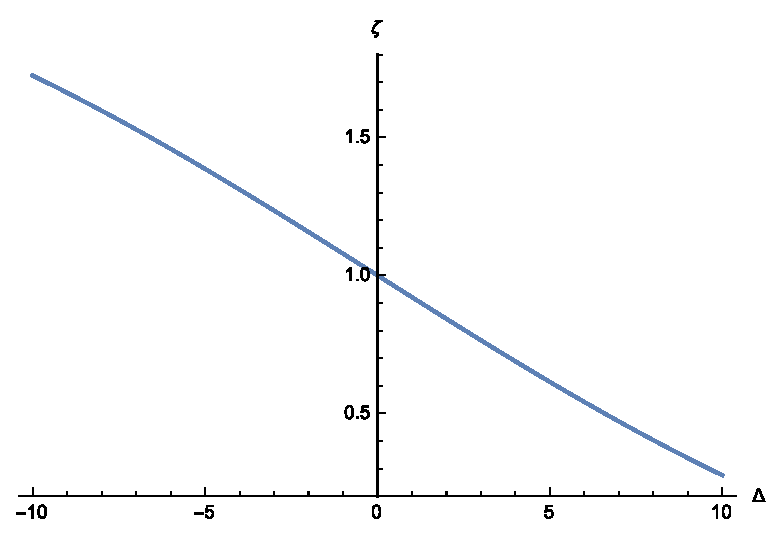
\includegraphics[scale = .8]{DF.eps}
		\caption{Expected Supply Damping Function}
		\end{center}
	\end{figure}

When delta is negative and the agent has overproduced, the agent will modify their future expectations by $\zeta > 1$. In the opposite situation, and the agent has underproduced, they will modify their future expectations by $\zeta < 1$. As the solution approaches steady state, $\delta$ will converge to zero and $\zeta$ converges to unity (\cref{results1}). 

	\begin{figure}[ht!]
		\begin{center}
		\includegraphics[scale = .6]{feedbackloop.png}
		\caption{Block Diagram of Feedback Loop}
		\label{feedback}
		\end{center}
	\end{figure}

 \Cref{feedback} details how the negative feedback loop is implemented. The optimization routine takes expected supply as an input and finds the optimal production bundle based on these expectations. After bid submission, the comparator finds the difference in expectation vs. reality and sends the result to the damping function. The damping function in-turn, creates a suitable damping ratio and multiplies it to the previous expectations to create future expectations. 

 	\begin{equation}
 		Q_{t+1}^{exp} = \zeta Q_{t}^{exp}
 	\end{equation}


% =========================================================== % 

\section{Achieved Results}
The first series of tests consisted of two agents, each with different utility coefficients, available assets, and cost structures. Agent \emph{1} is the larger of the two producers, and has the majority of its production capacity in natural gas. There are differences in the utility coefficients, however they are not extreme.\footnote{Recall that the closer the costs and coefficients are, the faster steady state will be reached}

	\begin{figure}[ht!]
		\begin{center}
		\includegraphics[scale = .25]{results.png}
		\caption{Summary of Results, Case 1}
		\label{results1}
		\end{center}
	\end{figure}

\Cref{results1} shows the results of the baseline simulation. Here, you can see that $ \alpha $ quickly converges to unity as $\delta$ converges to nil. Agent \emph{1}, the larger of the two producers, becomes the dominate player in the market with approximately 70\% market share. \*


\subsection{Handling Market Expansion}
The model is expandable and can handle an arbitrary number of players in the market. However, as the number of agents increases, the amount of iterations required to reach a steady state increases too, as the damping function must now incorporate two variable outputs. Numerically, the model becomes more sensitive to intial conditions and less stable. \footnote{Here stability refers the ability for the algorithim to converge to its limit} how  as a result, requiring the agent`s intial conditions to be closer together. 


\subsection{Effects of Taxation on Producers of Different Scales}
HERE IM GOING TO RUN SIMULATIONS SHOWING HOW THE MARGINAL TAX WILL DISPROPORTIONALLY EFFECT PRODUCERS OF DIFFERENT SCALES

\section{Conclusions}
WHAT CAN I INFER FROM THE ABOVE?

\newpage
% ==========================APPENDIX========================== % 
\appendix

	\section{WireFrame}

		\begin{figure}[ht!]
			\begin{center}
			\includegraphics[scale = .6]{wire.png}
			\end{center}
		\end{figure}




% ==========================BIB========================== % 


\newpage

\begin{thebibliography}{1}

	\bibitem{co2} EIA. ”How Much Carbon Dioxide (CO2) Is Produced hen Different Fuels Are Burned?”” U.S Energy Information Administration. U.S Energy Information Administration, n.d. Web. 9 Dec.2013.



\end{thebibliography}



\end{document} 
